\chapter{Research Design and Shared Methodology}
\label{ch:methodology}

\section{Relationship Between the Research Questions and Case Studies}
The five studies address the representation and fusion questions (SQ1 and SQ2) by comparing predictors on the same target and assessment units within each study. For robustness (SQ3), REASSEMBLE and MSM compare learned fusion under controlled input degradation. HANDOVER evaluates degradation and known input loss for the simpler baselines. PHM leaves the robustness of visual--sensor fusion open, and the ViFailback analysis includes no completed stress results for the reported fusion models. For SQ4, the evidence includes target validity in regression, probability quality and threshold outcomes in classification, and estimates of uncertainty or computational cost where available.

The five implemented studies carry the original welding question into tasks with different prediction targets. In PHM, photographs define the gear-condition proxy that sensor models predict. REASSEMBLE provides the principal comparison on completed robotic actions. MSM tests the procedure on abnormal milling intervals. ViFailback tests complete manipulation episodes across held-out tasks and separately examines transfer of a visual encoder. In HANDOVER, video and force--torque signals cover a common observation window for each labelled trial. The official test split supports evaluation of single-input predictors and fixed averaging. Fitting the proposed learned fusion model would also require participant identifiers for constructing training predictions (Appendix~\ref{app:handover}).

Figure~\ref{fig:research-workflow} shows how the welding objective relates to the five experiments. Each comparison required a defined target, paired observations and an assessment group appropriate to that target.
\begin{figure}[htbp]
\caption{Workflow for Data Qualification and Model Evaluation}\label{fig:research-workflow}
\centering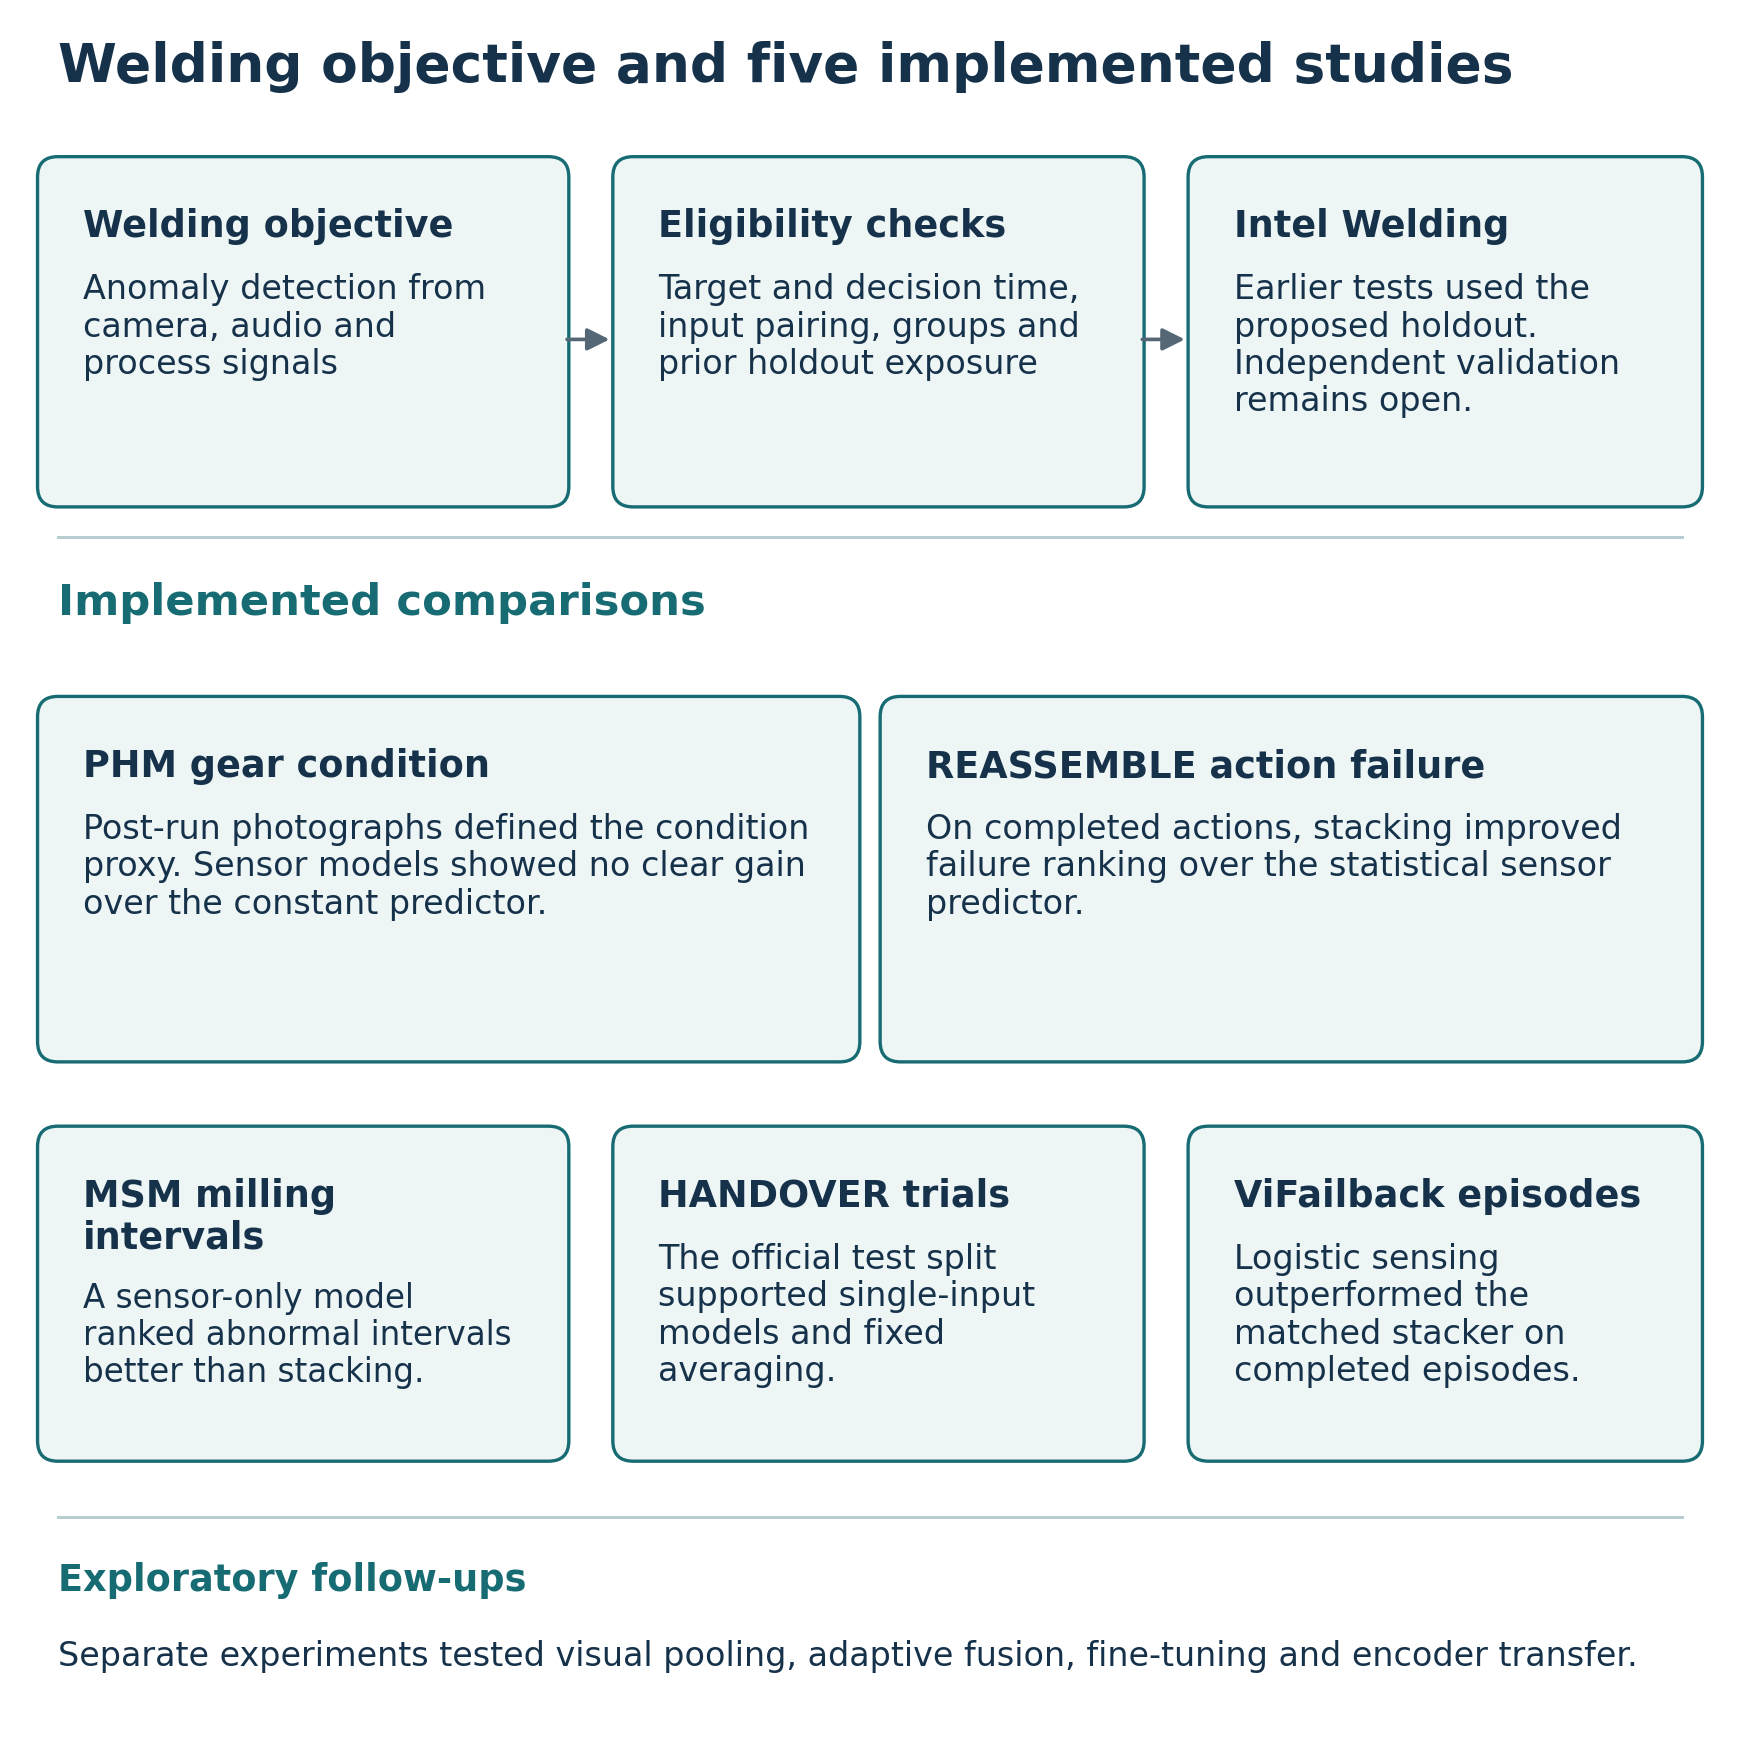
\includegraphics[width=\textwidth]{figures/research_workflow.png}
\displaynote{The five studies used different prediction targets. Each finding refers to the comparison within that study.}
\end{figure}

\section{Dataset Selection Criteria and Research Chronology}
Selection considered access, relevant physical observations, interpretable targets, correspondence, group identifiers, class support, and computational feasibility. These criteria changed what could be evaluated. A public multimodal dataset may lack a usable target for the proposed task; another may have labels but too few independent groups for the desired evaluation.

The initial welding proposal preceded the PHM and REASSEMBLE studies. Later investigations addressed uncertainties exposed by those studies: stronger sensor references, visual pooling, fine-tuning budgets, quality-conditioned fusion, and external adaptation. The October alignment record retained the original four-question hierarchy after a narrower quality-gate investigation had been considered. Follow-ups motivated by observed outcomes were exploratory. Appendix~G summarizes the scientific chronology.

The experimental inventory identifies the completed comparisons and their source records. For ViFailback these cover the original frozen study and the matched frozen and donor-backbone comparisons. The computational budget at thesis freeze placed target-CNN fine-tuning and the SQ3 corruption evaluation outside the final scope. The source manifest identifies the inspected Git commit \texttt{e32ec43aef69cc58adff0ea91e508308041598c5} and records hashes for selected files, including uncommitted report outputs.\ev{Remote source manifest}{\EvidenceRef{E111}{}, \EvidenceRef{E109}{}}

\section{Intel Welding Feasibility Assessment and Resulting Scope Decisions}
The Intel foundation scripts inspect sample structure, readability, timing/session fields, and duplicates. Their configuration disables a final test, and the audit encodes that earlier context evaluation had exposed the proposed holdout population. Reusing that population would preclude an independent confirmatory test. The retained subset does not establish the full original label mapping or a completed native multimodal classifier. Earlier contextual baseline reports therefore provide historical feasibility information, rather than evidence that a proposed Transformer-fusion architecture failed empirically.\ev{Intel Welding feasibility assessment}{\EvidenceRef{E019}{inspect\_sample, audit\_split, main}, \EvidenceRef{E018}{}, \EvidenceRef{E003}{section 3.1}}

The project record attributes the shift to PHM and REASSEMBLE to an agreement with the supervisor reported by the researcher. The two studies address the original architectural and evaluation questions using different tasks, modalities, and targets. No claim of welding deployment or welding-domain validation follows from success in robotic assembly or milling.

\section{Dataset Admission and Preparation Checks}
Admission requires an explicit sample manifest. Each row should identify its prediction unit, target source, physical group, input paths, interval boundaries, availability, and any exclusion reason. Visual checks cover decoding, frame support, geometry, and the distinction between visible context and visible target evidence. Sensor checks cover channel ordering, units, timestamps, gaps, duplicated rows, missing values, and the meaning of interpolation or aggregation. Pairing checks ask whether the two inputs describe the same event, not merely whether both files exist.

An exclusion is consequential when it changes the target distribution or removes difficult failures. Counts before and after exclusion are therefore part of the evaluation. Quarantined samples retain their original labels. In MSM, timing-alias correction and grouping support determine admission; in ViFailback, duplicate or invalid telemetry and video failures affect the cohort. Technical quality control cannot independently validate semantic labels, physical damage, or a camera's visibility of the relevant phenomenon.

\section{Target Provenance, Prediction Units, and Available Inputs}
A task record states what is being predicted, how the reference is obtained, and which inputs would be available at the prediction time. PHM's image-derived candidate-area score is a provisional condition proxy. Sensor prediction of that score measures agreement with the construction, not verified wear or remaining useful life. REASSEMBLE labels complete action outcomes. ViFailback labels complete episodes. MSM uses a declared mapping of milling labels, with alternatives treated as sensitivity analyses. The physical interpretation of a score depends on these definitions.

The observation horizon is explicit. Sampling frames from the entire action allows retrospective recognition of its outcome; it does not demonstrate warning before that outcome. Likewise, controller aggregates can summarize an interval only after it has elapsed. A prospective experiment would need a fixed decision time, causal preprocessing, a definition of lead time, and labels aligned to that horizon. The offline classifications do not measure lead time.

Process identity, duration, time index, or extraction latency can become predictive shortcuts. The PHM visual head receives extraction latency alongside its image features. A process-context gate may exploit action-specific prevalence, so its improvement would not automatically show that it recognized physical sensor reliability. Relevant context-only and constant-adjustment controls test narrower alternatives where available.

\section{Grouping, Data Splits, and Leakage Prevention}
The split unit determines the scope of the generalization claim. The principal PHM sensor protocol holds out gear experiments, REASSEMBLE groups actions by recording, MSM examines experiment and date groupings, and ViFailback separates tasks. HANDOVER retains the published trial partitions. The available identifiers allow neither independent verification of the reported participant separation nor construction of participant-disjoint inner folds. For MSM, a date can span multiple tools or operators, and physical equipment may recur across dates. A claim about a new machine or factory requires grouping information at that level.

Within an outer split, feature scaling, imputations estimated from data, model selection, calibration, thresholds, and fusion fitting must use training-side information. For stacking, the training bank contains predictions from models that did not fit the corresponding labels. If a branch recipe is selected, that selection also belongs inside the permitted training hierarchy. Even with an out-of-fold prediction head, assessment information can enter the model through an encoder or normalizer fitted on the full dataset. Each base prediction for the original REASSEMBLE stacker came from a branch fitted without data from the corresponding recording. Within each outer split, internal stacker validation reused the same out-of-fold (OOF) prediction bank built from the outer training recordings. A branch that supplied a prediction for a stacker training row could have been fitted on recordings held out for that stacker validation split. The outer-assessment recordings remained excluded from fitting. Full independence at the deeper validation stage has yet to be demonstrated. This dependency limits the claim of strict nesting.\ev{Original stacker-validation dependency}{\EvidenceRef{E004}{section 15.4}}

The original REASSEMBLE cohort comprises 4,530 actions, 509 failures, and 148 recordings. Its five held-out partitions together cover this population. A later 753-action comparison uses one of these exposed outer partitions, not a new external holdout. Cohort reconciliation uses sample and recording identities to distinguish overlapping and identical populations. An earlier summary listed 28 recordings. The sample identifiers establish that this subset contains 26.\ev{Assessment sample and recording identifiers}{\EvidenceRef{E052}{}}

A specific PHM four-arm runner fits a normalizer before a loop that changes the held-out experiment. Its held-out experiments therefore contribute to preprocessing. The principal PHM runner fits its normalizer inside each fold. A fold-isolated estimate for the four-arm comparison would require repeating that experiment.

\section{Model Fitting, Selection, Calibration, and Threshold Procedures}
Each comparison defines trainable components, initialization, selection candidates, training budget, and stopping rules. An epoch count alone does not establish matched optimization if samples, batch sizes, early stopping, or cached representations differ. The experimental programme included original comparisons, exploratory pilots and matched short-budget diagnostics. Some larger experiments completed only a subset of the planned fits.

Calibration maps raw model scores to probabilities using training-side predictions. Discrimination and calibration are different properties: a monotonic score transformation can preserve ranking while changing probability errors. The core branch calibrators use sigmoid logistic maps on selected inner out-of-fold scores. The original softmax gates have no free final intercept or post-gate calibrator, whereas F2 has a free intercept and no additional post-stacker calibration. These function-class and post-processing choices remain visible in the comparison \citep{Guo2017Calibration}.

A decision threshold is selected using permitted training predictions and a stated objective, such as balanced accuracy. The original implementation searches a grid from .01 to .99. Such a threshold is a protocol choice, not a cost-optimized industrial alarm policy. At that threshold, sensitivity, specificity, precision, and false-alert burden give a clearer account of performance than accuracy alone. Assessing operational acceptance also requires information about stakeholder costs.

\section{Metrics and Uncertainty Estimation}
For regression, MAE is $n^{-1}\sum_i|y_i-\hat y_i|$ and RMSE is $\sqrt{n^{-1}\sum_i(y_i-\hat y_i)^2}$. Both inherit the units and validity of the target. $R^2$ compares squared error with a reference denominator and can be unstable or negative in small held-out groups. Tooth-level and run-level PHM metrics remain separate because their targets and dependence differ.

For classification, the main ranking statistic is average precision as implemented by \texttt{average\_precision\_score}. With recall increments $\Delta R_k$ and precision $P_k$, $\mathrm{AP}=\sum_k\Delta R_kP_k$. It is not the same numerical quantity as trapezoidal area under a precision--recall curve. AUROC measures ranking over negative--positive pairs; AP depends strongly on the positive-class prevalence. Precision--recall analysis is particularly useful for imbalanced outcomes, but scores from different prevalences should not be treated as a model ranking across datasets \citep{Saito2015PrecisionRecall}.

Binary failure AP, success AP, their macro average, mean-fold AP, and AP computed from pooled held-out predictions are different estimands. The nonlinear metric implies that mean-fold AP generally differs from pooled AP. ViFailback tables name macro AP explicitly; REASSEMBLE's original headline uses pooled failure AP. Threshold metrics and Brier score $n^{-1}\sum_i(p_i-y_i)^2$ address different questions. Interpret calibration summaries in light of how the bins were defined and how many observations contributed.

For a paired model comparison, define $\Delta=\mathrm{AP}(p_A,y)-\mathrm{AP}(p_B,y)$ on identical rows. A cluster bootstrap samples dependence groups with replacement and recomputes the paired difference. Core REASSEMBLE reports use 2,000 recording-level replicates; a PHM report uses 10,000 run-cluster replicates over 20 runs. These are intervals conditional on the saved fitted models and the chosen resampling unit. They do not capture all retraining, model-selection, seed, or new-site uncertainty. Five MSM dates provide a particularly small basis for a date-cluster interval. Cross-validation folds are overlapping training experiments, not independent replications; uncertainty should not be inferred from a naive standard error over folds \citep{Bengio2004CVVariance}.

\section{Robustness Evaluation Design}
A robustness test specifies how the failure occurs, which modality and stage it affects, and how severe it is. It also reports the number of realizations, any exposure to the failure during training, and the observations and metric used. The availability mask identifies a stream declared missing. A corrupted stream can remain available and supply a prediction. Corrupting pixels targets a different stage from corrupting cached visual features. Sensor corruption can affect raw channels, statistics, or logits. Recompute any quality features meant to describe the corrupted observation.

Clean and degraded absolute scores are both needed. A smaller clean-relative drop can coexist with worse absolute performance. A gate can shift weight away from a corrupted modality while still underperforming the intact unimodal predictor. The relevant controls include the surviving branch, a static fusion model with matched augmentation exposure, and any simpler parameterization needed to isolate adaptation. Training with modality dropout establishes exposure to missing inputs. Recovery is measured on held-out cases where the input is absent.

The original two-input gate routes a single surviving branch with weight one. With fixed branch outputs this makes single-input predictions identical regardless of gate training. Both missing inputs raise an error; no predictive result is attributed to that state. These tests leave open the effects of clock offsets, previously unseen machines and novel failure mechanisms.

\section{Reproducibility and Experiment Provenance}
The core REASSEMBLE visual branch loaded the pretrained RT-DETR-R18vd checkpoint through Hugging Face Transformers and selected its ResNet18-vd convolutional backbone. The backbone stayed frozen while a separate binary classifier learned from its pooled features. The same library supplied the PatchTST sensor encoder, initialized from scratch \citep{Wolf2020Transformers}. PyTorch trained the neural prediction heads with AdamW \citep{Paszke2019PyTorch}. Scikit-learn supplied the grouped stratified splits and logistic regression baseline \citep{Pedregosa2011ScikitLearn}. The PHM image regressor used the Ultralytics RT-DETR-L prediction path to extract intermediate feature maps \citep{UltralyticsRTDETR}.\ev{Library use in executed models}{\EvidenceRef{E064}{}, \EvidenceRef{E065}{}, \EvidenceRef{E067}{}, \EvidenceRef{E046}{}, \EvidenceRef{E033}{}, \EvidenceRef{E004}{P01}}

Verification used archived source code, configurations and results. Where saved predictions were available for selected comparisons, metrics could also be recalculated. These checks used the existing fitted models' outputs without retraining or rerunning inference on raw observations. For historical runs, the recorded configuration and results identify which code path produced the reported comparison.

The evidence files record source paths and hashes for the inspected implementation, the assessment cohorts and the metric definitions. Literature extraction records connect bibliographic metadata and relevant passages to individual publications.

\section{Computational Constraints and Exploratory Versus Confirmatory Analysis}
Resource limits motivated cached features, compact heads, small selection grids, and bounded follow-ups. Those choices define the tested system. They cannot justify declaring an undertrained architecture intrinsically unsuitable or an unfinished arm inferior. Timings must state whether they measure warm extraction, a head fit, or an end-to-end pipeline, with device and preprocessing included where available.

The work is primarily exploratory and retrospective. Repeated exposure to the same assessment cohort, follow-ups selected after inspecting results, and later protocol adjustments limit confirmatory interpretation. A future confirmatory study should freeze targets, cohort construction, selection rules, primary contrasts, corruption operators, and claim criteria before the assessment is opened. The conclusions are conditional on this exploratory development history and on the saved evidence available for each study.
